
%\documentclass[a4paper]{jsbook}
%\usepackage{mcmd_jp}
%\begin{document}

\section{msortf レコードの並べ換え\label{sect:msortf}}
\index{msortf@msortf}
\verb|f=|パラメータで指定した項目を基準にして、レコードを並べ換える。\\
ソーティングアルゴリズムはquick sortを利用しており、
安定ソート(キーの値が同じ行については元の順序を保存する)にはならないことに注意する。\\
出力CSVの項目名の後ろには、並び順情報として\verb|%|で始まる文字列が付加される。
書式は\verb|%優先順位[並び順]|で、
詳細は以下、\verb|f=|パラメータを参照のこと。

\subsection*{書式}
\verb|msortf f= [pways=] [maxlines=] [blocks=] [threadCnt=] [-noflg]|
\hyperref[sect:option_i]{[i=]}
\hyperref[sect:option_o]{[o=]}
\hyperref[sect:option_assert_diffSize]{[-assert\_diffSize]}
\hyperref[sect:option_nfn]{[-nfn]} 
\hyperref[sect:option_nfno]{[-nfno]}  
\hyperref[sect:option_x]{[-x]}
\hyperref[sect:option_tmpPath]{[tmpPath=]} 
\hyperref[sect:option_precision]{[precision=]}
\verb|[-params]|
\verb|[--help]|
\verb|[--helpl]|
\verb|[--version]|\\

\subsection*{パラメータ}
\begin{table}[htbp]
%\begin{center}
{\small
\begin{tabular}{ll}
\verb|i=|    & 入力ファイル名を指定する。\\
\verb|o=|    & 出力ファイル名を指定する。\\ 
\verb|f=|    & レコードを並べ換える基準となる項目名リストを指定する。\\
             & 並び順は、数値/文字列、昇順/降順の組み合せで4通り指定できる。\\
             & 指定方法は\verb|%|に続けて\verb|n|と\verb|r|を以下の通り組み合わせる。\\
             & 文字列昇順:\verb|項目名|(\verb|%|指定なし)、文字列逆順:\verb|f=項目名%r|、数値昇順:\verb|f=項目名%n|、数値降順:\verb|f=項目名%nr|。\\
\verb|-noflg| & 出力CSVのヘッダーにソーティングの印(\verb|%0,%0n|など)を付けない。\\
%\verb|pways=| & 分割ソートにおいていくつのファイルを同時に併合するかを指定する(デフォルト:32)。\\
%\verb|maxlines=| & 分割ソートにおける一つの分割ファイルの行数上限(デフォルト:500000)。\\
%\verb|blocks=| & 分割ソートにおける一つの分割ファイルのブロック数上限(デフォルト:10)。1ブロックはデフォルトで4MBで、環境変数\verb|KG_iSize|によって変更可能。\verb|maxlines=|と\verb|blocks=|のいずれかの上限に達した時に、そこまでに読み込んだデータをメモリ内でソートし、分割ファイルに書き出す。\\
%\verb|threadCnt=| & 分割ソートにおける並列処理スレッド数(デフォルト:8)。\\

\verb|pways=|    & 同時併合ファイル数([2-100]:デフォルト32)【任意】\\
                 & 分割ソートされた複数のファイルを同時に何個併合するかを指定する。\\
\verb|blocks=|   & バッファブロック数([1-1000]:デフォルト10)【任意】\\
                 & メモリ内でソートする際のメモリサイズ上限をブロックサイズで指定する。\\
                 & 1ブロックは入力バッファサイズ×4で、デフォルトは4MB。\\
\verb|maxlines=| & メモリソートレコード件数上限([100-1000万]:デフォルト50万)【任意】\\
                 & メモリ内でソートする際の件数の上限を指定する。\\
                 & データの一行あたりの平均サイズに応じて、
                   \verb|blocks=|制限と\verb|maxlines=|制限のいずれかが使われる。\\
\verb|threadCnt=|& メモリ内でソートを実行するthread数 ([1-50]:デフォルト8)【任意】\\
& 分割ソートする際に、マルチスレッドの機能を用いて同時にソートする数を指定する。\\


\end{tabular} 
}
\end{table}
 
\subsection*{備考}
\begin{enumerate}
\item \verb|f=|で、文字列項目に対して\verb|%n|を指定した場合の動作は不定である。
\item \verb|f=|を省略した場合は\verb|i=|で指定したファイルを順番に併合する(\hyperref[sect:mcat]{mcat}と同様)。
\item キー項目ににNULL値が含まれる場合、NULL値はどのような値よりも小さい値として扱われる。
%\item \verb|i=|で指定したファイルは全て存在し、また項目名は全て同じであることを前提としており、\verb|mcat|のような柔軟な指定はできない。
\item \verb|f=a,a|のように同じ項目を2つ以上指定した場合、最初に指定した項目のみが有効となり、2番目以降に指定した項目は無視される。\verb|msortf f=a,a|は\verb|msortf f=a|と見なされ、\verb|msortf f=a,b,a,b|は\verb|msortf f=a,b|と見なされる。

\end{enumerate}

\subsection*{利用例}
\subsubsection*{Example 1: Basic example}

Sort by \verb|item| and \verb|date|.


\begin{Verbatim}[baselinestretch=0.7,frame=single]
$ more dat1.csv
item,date,quantity,price
B,20081201,4,40
A,20081201,10,200
A,20081201,10,100
B,20081203,5,50
B,20081201,2,500
A,20081201,3,300
$ msortf f=item,date i=dat1.csv o=rsl1.csv
#END# kgsortf f=item,date i=dat1.csv o=rsl1.csv
$ more rsl1.csv
item%0,date%1,quantity,price
A,20081201,10,200
A,20081201,10,100
A,20081201,3,300
B,20081201,4,40
B,20081201,2,500
B,20081203,5,50
\end{Verbatim}
\subsubsection*{Example 2: Sort by quantity in descending order and price in ascending order.}



\begin{Verbatim}[baselinestretch=0.7,frame=single]
$ msortf f=quantity%nr,price%n i=dat1.csv o=rsl2.csv
#END# kgsortf f=quantity%nr,price%n i=dat1.csv o=rsl2.csv
$ more rsl2.csv
item,date,quantity%0nr,price%1n
A,20081201,10,100
A,20081201,10,200
B,20081203,5,50
B,20081201,4,40
A,20081201,3,300
B,20081201,2,500
\end{Verbatim}



\subsection*{CSV特殊文字と並び順についての注意}
msortfではCSVの特殊文字を解釈して並べ替えを行う為に、
CSVの特殊文字であるカンマとダブルクォーツを含むデータについては
UNIXのsortコマンドの実行結果と異なることがある。
例えば、以下に示すような第一項目に
a(0x61)、NULL値、スペース文字(0x20)、+(0x2b)、-(0x2d)、
カンマ(0x2c)、ダブルクォーツ(0x22)を持つデータについて見てみよう。
カンマとダブルクォーツはCSVの特殊文字のため特別な表記となっている。
また表示上の分かりやすさのために第二項目f2として全行に"x"を付加している。\\

\begin{Verbatim}[baselinestretch=0.7,frame=single,fontsize=\small]
f1,f2
a,x
,x
 ,x
+,x
-,x
",",x
"""",x
\end{Verbatim}

このデータを「msortf f=f1」で並べ替えた結果は以下の通りで、
CSVフォーマットにおける特殊記号を考慮した上での本来の並び順
(NULL,スペース,ダブルクォーツ,+,カンマ,-,a)になっていることがわかる。\\

\begin{Verbatim}[baselinestretch=0.7,frame=single,fontsize=\small]
f1,f2
,x
 ,x
"""",x
+,x
",",x
-,x
a,x
\end{Verbatim}

\subsection*{ベンチマークテスト}
msortfの速度についてのベンチマークテストの結果を示す。
入力データは以下に示すような6項目からなるデータである。
全ての項目は一様乱数により生成されている。\\

\begin{Verbatim}[baselinestretch=0.7,frame=single,fontsize=\small]
key,fld1,fld2,fld3,fld4,fldn
95547922,162,159,192,118,74
81438069,138,157,155,122,58
26885062,129,199,133,198,75
32651684,180,107,123,170,-14
10245631,164,103,159,154,-63
15145156,182,191,175,107,-60
29254245,188,185,129,124,5
85423170,116,164,175,113,57
55155879,105,163,195,167,25
66997216,195,139,195,113,39
.
.
\end{Verbatim}

\subsection*{キー項目の値の種類数および状態に関する比較}
レコード数を100万件とし、
キー(key項目)の値の種類を2、10、100、1000、10000とした場合の結果を表\ref{tbl:msortf:bench}に示す。
また、表中の(1),(2)をグラフ化したものが図\ref{fig:msortf:bench1}に、
また(4),(5)をグラフ化したものが図\ref{fig:msortf:bench2}に示されている。

「乱数」項目は乱数の上限を最大とした場合の乱数値をキーとしている。
また「乱数昇順(降順)」は、「乱数」データを事前に昇順(降順)に並べ替えたデータである。
msortf以外に、比較の為にMUSASHIのxtsortコマンド、
およびUNIXのsortコマンドの結果も示す。
「sort -k1」は、第1番目の項目で並べ替えた結果である。
また上三行はmsortf、xtsort、sortの各コマンドで第1番目の項目を
文字列として並べ替えた時の結果であり、
下三行は数値として並べ替えたときの結果である。
実行環境は、MacBookPro, Mac OS X 10.9.1, 2.6GHz Intel Core i7, 16GB メモリ、である。

\begin{table}[hbt]
\begin{center}
\caption{Comparison of types of key values and its condition among various sort commands}
\begin{tabular}{clrrrrrrrr}
\hline
No. & Command & 2 Types & 10 Types & 100 Types & 1000 Types & 10000 Types & Rand & Rand Asc & Rand Desc \\
\hline
(1)&msortf f=key&0.29&0.33&0.37&0.40&0.43&0.50&0.29&0.28 \\
(2)&xtsort -k key&1.25&1.24&1.22&1.20&1.19&1.12&0.85&1.00 \\
(3)&sort -k1&16.96&16.63&16.05&15.56&15.08&13.68&6.85&7.13 \\
\hline
(4)&msortf f=key\%n&0.46&0.56&0.65&0.72&0.79&1.02&0.59&0.59 \\
(5)&xtsort -k key\%n&2.52&2.72&2.96&3.16&3.21&3.22&2.31&2.32 \\
(6)&sort -k1 -n&16.65&14.52&11.54&8.56&5.71&0.95&0.33&0.36 \\
\hline
\end{tabular}
\end{center}
\end{table}


\begin{figure}[!hbt]
\begin{center}
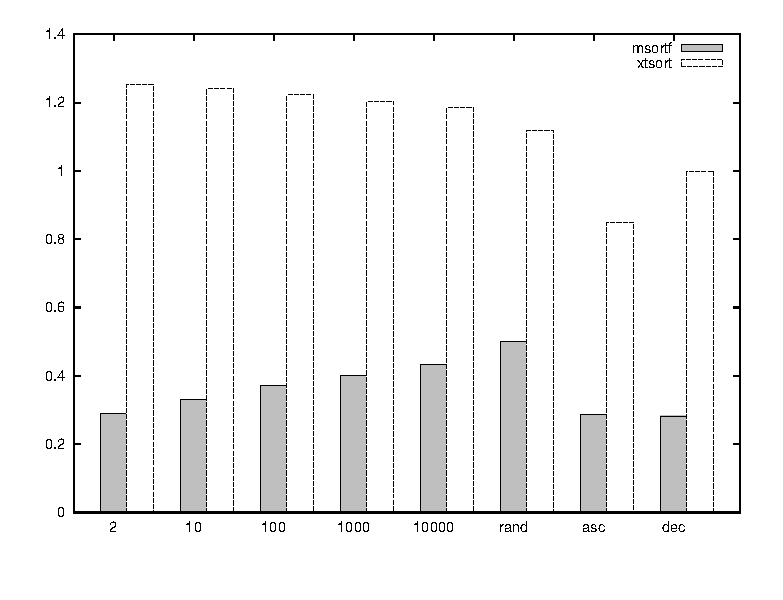
\includegraphics[scale=.8]{figure/msortf/key.eps}
\end{center}
\caption{キーの種類数別に見るmsortf,xtsortの文字列ソートの比較(横軸がキーの種類数,縦軸が秒数)\label{fig:msortf:bench1}}
\end{figure}

\begin{figure}[!hbt]
\begin{center}
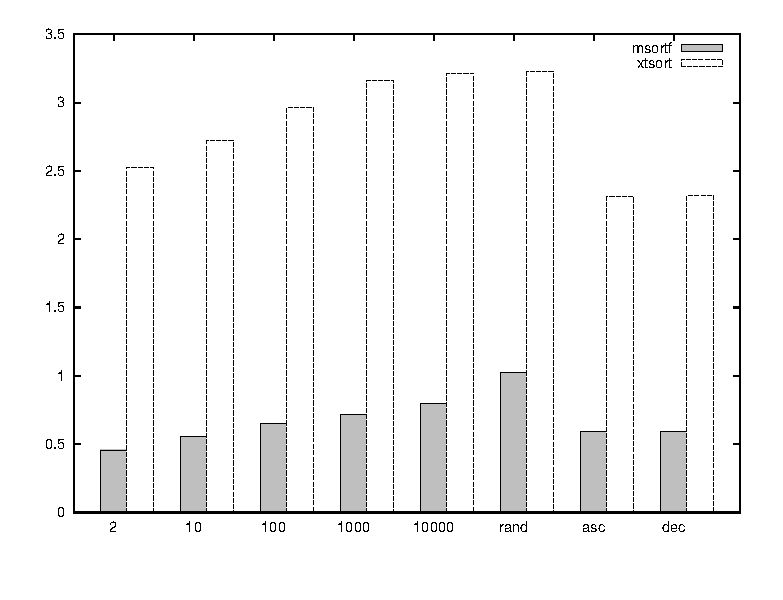
\includegraphics[scale=.8]{figure/msortf/num.eps}
\end{center}
\caption{キーの種類数別に見るmsortf,xtsortの数値ソートの比較(横軸がキーの種類数,縦軸が秒数)\label{fig:msortf:bench2}}
\end{figure}

msortfはxtsortより2倍〜5倍高速である。sortについては、条件にもよるが数十倍高速である。
MUSASHIのsortとで利用しているquick sortのアルゴリズムは全く同じであるが、
MCMDにおいては分割ソートにおいてマルチスレッドを使い並列処理している。
その影響の差が出ているということであろう。
%msortはキーの種類が多い場合、および事前にソート済みのデータに対してmsortfより良い性能を示している。
%msortでは入力データを内部で項目で分割せず行単位でソートするため、
%第1項目の値の種類数が少ないと、
%その項目だけで大小関係が決まらず次の項目も比較しにいくため
%比較に余分な比較のオーバーヘッドがかかっていると考えられる。
%また項目数が多いデータではmsortfより高速に動作するであろう。
%ただし、他のコマンドへの入力データのキー項目をmsortでソートする場合、
%十分注意して利用しなければ正しい結果が得られないことがある。
%詳しくはmsortのマニュアルを参照のこと。\\
%一方で数値ソートについては、msortfはxtsortより2倍程度効率的である。
%乱数データやソート済みデータについては
次に、キーの種類数を100および最大に固定し、
データ件数を100万件から1000万件まで変化させた時の文字ソートの速度について実験した。
ここではmsortf、xtsortの2つのコマンドの比較を図\ref{fig:msortf:bench3},\ref{fig:msortf:bench4}に示す。

\begin{figure}[!hbt]
\begin{center}
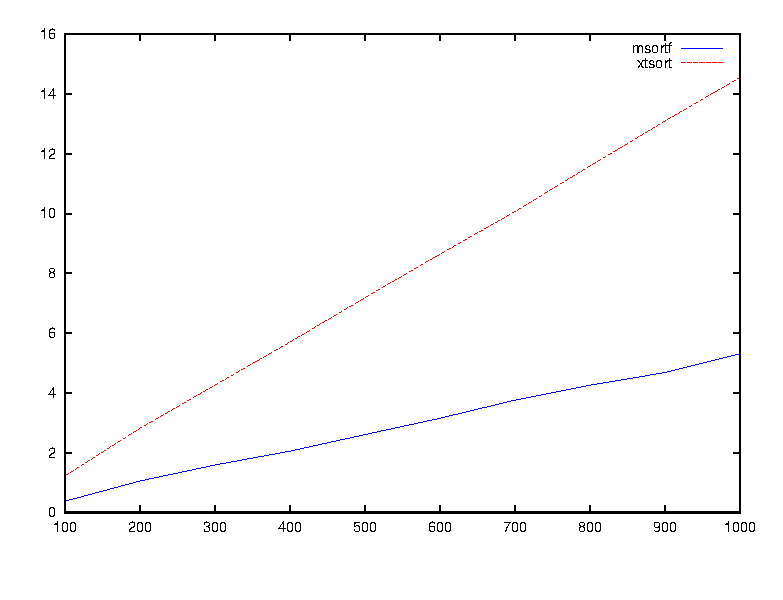
\includegraphics[scale=.8]{figure/msortf/line_100.eps}
\end{center}
\caption{キーの種類数を100とした場合の結果(横軸がデータ件数,縦軸が秒数)\label{fig:msortf:bench3}}
\end{figure}

\begin{figure}[!hbt]
\begin{center}
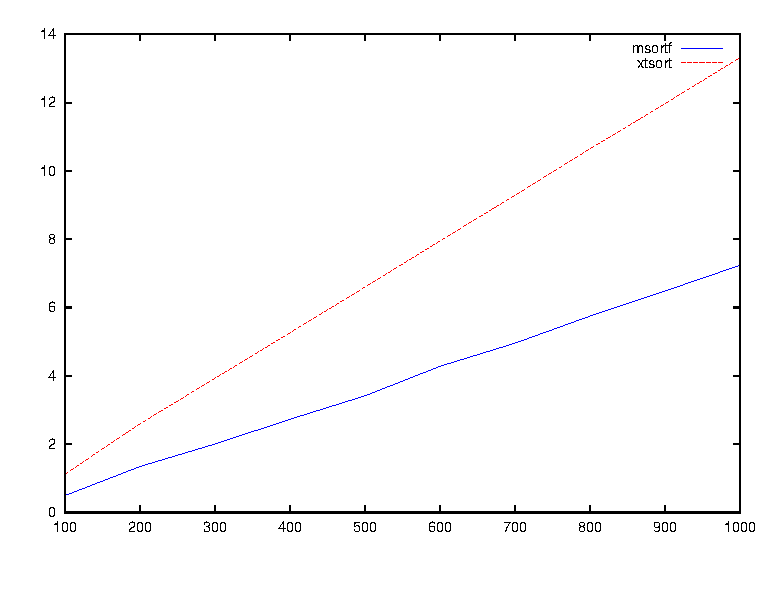
\includegraphics[scale=.8]{figure/msortf/line_rand.eps}
\end{center}
\caption{キーの種類数を乱数(最大)とした場合の結果(横軸がデータ件数,縦軸が秒数)\label{fig:msortf:bench4}}
\end{figure}

\subsection*{関連コマンド}
%\ref{sect:msort} msort

%\end{document}
